% Created 2017-03-22 Wed 20:07
% Intended LaTeX compiler: pdflatex
\documentclass[presentation]{beamer}
\usepackage[utf8]{inputenc}
\usepackage[T1]{fontenc}
\usepackage{graphicx}
\usepackage{grffile}
\usepackage{longtable}
\usepackage{wrapfig}
\usepackage{rotating}
\usepackage[normalem]{ulem}
\usepackage{amsmath}
\usepackage{textcomp}
\usepackage{amssymb}
\usepackage{capt-of}
\usepackage{hyperref}
\usetheme{CambridgeUS}
\usecolortheme{beaver}
\setcounter{secnumdepth}{1}
\author{Zheng Tian}
\date{}
\title{Lecture 6: Linear Regression with One Regressor}
\hypersetup{
 pdfauthor={Zheng Tian},
 pdftitle={Lecture 6: Linear Regression with One Regressor},
 pdfkeywords={},
 pdfsubject={},
 pdfcreator={Emacs 25.1.1 (Org mode 9.0.3)}, 
 pdflang={English}}
\begin{document}

\maketitle
\begin{frame}{Outline}
\setcounter{tocdepth}{1}
\tableofcontents
\end{frame}



\section{The Linear Regression Model}
\label{sec:orgc95fee2}

\begin{frame}[label={sec:org9913858}]{Definition of \alert{regress} in Merriam-Webster's dictionary}
Merriam-Webster gives the following definition of the word "regress":
\begin{enumerate}
\item An act or the privilege of going or coming back
\item Movement backward to a previous and especially worse or more
primitive state or condition
\item The act of reasoning backward
\end{enumerate}
\end{frame}

\begin{frame}[label={sec:org4346fcf}]{The meaning of regression in statistics?}
\begin{itemize}
\item In statistics, regression analysis focus on the conditional mean of the
dependent variable given the independent variables, which is a
function of the values of independent variables.

\item A very simple functional form of a conditional expectation is a linear
function. That is, we can model the conditional mean as follows,

\begin{equation}
\label{eq:genpopreg}
\mathrm{E}(Y \mid X = x) = f(x) = \beta_{0} + \beta_1 x
\end{equation}

The above equation is a \alert{simple linear regression function}.
\end{itemize}
\end{frame}

\begin{frame}[label={sec:org13e6625}]{Research question:}
\begin{itemize}
\item Let's introduce a regression analysis with the application of test
scores versus class sizes in California school districts. 
\begin{quote}
Can reducing class sizes increase students' test scores?
\end{quote}

\item How can we answer this question?
\end{itemize}
\end{frame}

\begin{frame}[label={sec:org135efae}]{Randomized controlled experiment}
\begin{itemize}
\item Randomly choose 42 students and divide them into two classes,
with one having 20 students and another having 22.
\item They are
taught with the same subject and by the same teachers.
\item Randomization ensures that it is the difference in class sizes of
the two classes that is the only factor affecting test scores.
\end{itemize}
\end{frame}

\begin{frame}[label={sec:orgbe54642}]{Compute conditional means}
\begin{itemize}
\item Compute the expected values
of test scores, given the different class sizes.
\begin{gather*}
\mathrm{E}(TestScore | ClassSize = 20) \\
\mathrm{E}(TestScore | ClassSize = 22)
\end{gather*}

\item The effect of class size on test scores is
\begin{equation*}
\mathrm{E}(TestScore | ClassSize = 20) - \mathrm{E}(TestScore | ClassSize = 22)
\end{equation*}
\end{itemize}
\end{frame}

\begin{frame}[label={sec:org766c6d8}]{The population regression function for test scores on class sizes}
\begin{itemize}
\item We use a linear regression function to describe the relationship
between test scores and class sizes.

\item The \alert{population regression function} or the \alert{population regression
line}

\begin{equation}
\label{eq:popreg-testscore}
\mathrm{E}(TestScore | ClassSzie) = \beta_0 + \beta_1 ClassSize
\end{equation}
\end{itemize}
\end{frame}

\begin{frame}[label={sec:org2e2f1f2}]{The simple linear regression model for test scores on class sizes}
\begin{itemize}
\item We can lump all these factors into a single term, and set up a \alert{simple linear
regression model} as follows,

\begin{equation}
\label{eq:regmodel-testscore}
TestScore = \beta_0 + \beta_1 ClassSize + OtherFactors
\end{equation}

\item If we assume \(\mathrm{E}(OtherFactors | ClassSize) = 0\), then the
simple linear regression model becomes the population regression line.
\end{itemize}
\end{frame}

\begin{frame}[label={sec:org2bd2326}]{A distinction between the population regression function and the population regression model}
\begin{itemize}
\item A population regression function
\begin{itemize}
\item It's a deterministic relation between class size and the expectation of
test scores.
\item However, we cannot compute the exact value of the test score of a
particular observation.
\end{itemize}

\item A population regression model
\begin{itemize}
\item It's a complete description of a data generating process (DGP).
\item The association between test scores and class size is not
deterministic, depending on the value of other factors.
\end{itemize}
\end{itemize}
\end{frame}

\begin{frame}[label={sec:orgf33f8c6}]{An interpretation of the population regression model}
\begin{itemize}
\item Now we have set up the simple linear regression model,
\begin{equation*}
TestScore = \beta_0 + \beta_1 ClassSize + OtherFactors
\end{equation*}
What is \(\beta_1\) and \(\beta_0\) represent in the model?
\end{itemize}
\end{frame}

\begin{frame}[label={sec:orgefd4a62}]{Interpret \(\beta_1\)}
\begin{itemize}
\item Denote \(\Delta TestScore\) and \(\Delta ClassSize\) to
be their respective change.

\item \alert{Holding other factors constant}, we have
\[ \Delta TestScore = \beta_1 \Delta ClassSize  \]
where \(\beta_0\) is removed because it is a constant.

\item Then, we get

\[ \beta_1 = \frac{\Delta TestScore}{\Delta ClassSize} \]

That is, \(\beta_1\) measures the change in the test score resulting
from a \alert{one-unit change} in the class size.
\end{itemize}
\end{frame}

\begin{frame}[label={sec:org88c52ad}]{Marginal effect}
\begin{itemize}
\item When \(TestScore\) and
\(ClassSize\) are two continuous variable, we can write \(\beta_1\) as

\[\beta_1 = \frac{\mathrm{d} TestScore}{\mathrm{d} ClassSize}  \]

\item We often call \(\beta_1\) as the \alert{marginal effect} of the class
size on the test score.
\end{itemize}
\end{frame}

\begin{frame}[label={sec:org3f92ad1}]{Holding other things constant}
\begin{itemize}
\item The phrase of "holding other factors constant" is important. Without
it, we cannot disentangle the effect of class sizes on test scores
from other factors.
\item "Holding other things constant" is often expressed
as the notion of \alert{ceteris paribus}.
\end{itemize}
\end{frame}

\begin{frame}[label={sec:org5fe956b}]{Interpret \(\beta_0\)}
\begin{itemize}
\item \(\beta_0\) is the intercept in the model.
\item Sometimes it bears real
meanings, but sometimes it merely represents an intercept.
\item In regression model of test scores on class sizes, \(\beta_0\) is the
test score when the class size and other factors are all zero, which
is obviously nonsensical.
\end{itemize}
\end{frame}

\begin{frame}[label={sec:org51331bc}]{The general linear regression model}
\begin{itemize}
\item Consider two random variables \(Y\) and \(X\). For both, there are \(n\) observations so that
each observation \(i = 1, 2, 3, \ldots\) is associated with a pair of
values of \((X_i, Y_i)\).

\item Then a \alert{simple linear regression model} that associates \(Y\) with \(X\) is

\begin{equation}
\label{eq:single-regress}
Y_i = \beta_0 + \beta_1 X_i + u_i, \text{ for } i = 1, \ldots, n
\end{equation}

\item \(Y_i\) is called the dependent variable, the regressand, or the LHS
(left-hand side) variable.
\item \(X_i\) is called the independent variable, the regressor, or the RHS
(right-hand side) variable.
\end{itemize}
\end{frame}

\begin{frame}[label={sec:org58b4bc7}]{The general linear regression model (cont'd)}
\begin{itemize}
\item \(\beta_{0}\) is the intercept, or the constant term. It can either have
economic meaning or have merely mathematical sense, which determines
the level of the regression line, i.e., the point of intersection
with the Y axis.
\item \(\beta_{1}\) is the slope of the population regression line. Since
\(\beta_1 = \mathrm{d}Y_i/ \mathrm{d}X_i\), it is the marginal effect
of \(X\) on \(Y\). That is, holding other things constant, one unit
change in \(X\) will make \(Y\) change by \(\beta_1\) units.
\item \(u_i\) is the error term. \(u_i = Y_i - (\beta_0 + \beta_1 X_i)\)
incorporates all the other factors besides \(X\) that determine the
value of \(Y\).
\item \(\beta_{0} + \beta_{1}X_{i}\) represents the population regression
function(or the population regression line).
\end{itemize}
\end{frame}

\begin{frame}[label={sec:org8c6877b}]{An graphical illustration of a linear regression model}
\begin{figure}[htbp]
\centering
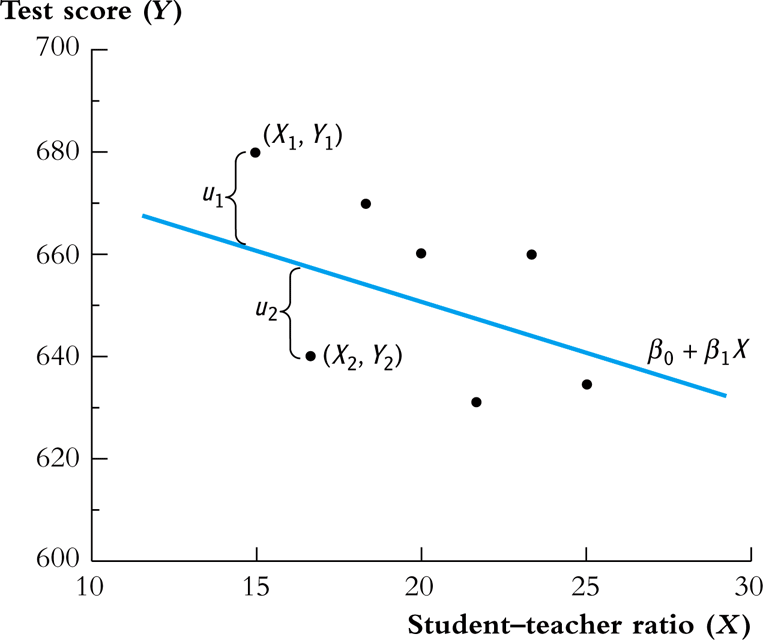
\includegraphics[width=0.75\textwidth]{figure/fig-4-1.png}
\caption{\label{fig:org0026493}
The Population Regression Line}
\end{figure}
\end{frame}



\section{The OLS Estimation Method for a Linear Regression Model}
\label{sec:org50e220c}

\begin{frame}[label={sec:orgb13f47f}]{The intuition for the OLS and minimization}
\begin{itemize}
\item We use the ordinary least squares (OLS) estimation method to estimate
the simple linear regression model. 
$$Y_i = \beta_0 + \beta_1 X_i + u_i, \text{ for } i = 1, \ldots, n$$
\end{itemize}
\end{frame}

\begin{frame}[label={sec:org730b56e}]{Ordinary}
\begin{itemize}
\item It means that the OLS estimator is a very basic method,
from which we may derive some variations of the OLS
estimator.

\item Other least squares estimators: the weighted least squares (WLS),
and the generalized least squares (GLS).
\end{itemize}
\end{frame}

\begin{frame}[label={sec:org0e56d08}]{Least}
\begin{itemize}
\item It means that the OLS estimator tries to minimize something. The
"something" is the mistakes we make when we try to guess
(estimate) the values of the parameters in the model.

\item If our guess for \(\beta_0\) and \(\beta_1\) is \(b_0\) and \(b_1\), then
the mistake of our guess is 
$$\hat{u}_{i} = Y_{i} - b_0 - b_1 X_i$$
\end{itemize}
\end{frame}

\begin{frame}[label={sec:org55afaf7}]{Squares}
\begin{itemize}
\item It represent the actual thing (a quantity) that we minimize. The
OLS does not attempt to minimize each \(\hat{u}_{i}\).

\item We minimize the sum of the squared mistakes, 
$$\sum_{i=1}^n \hat{u}_i^2$$
Taking square is to avoid possible offsetting
between positive and negative values of \(\hat{u}_i\) in \(\sum_i
  \hat{u}_i\).
\end{itemize}
\end{frame}

\begin{frame}[label={sec:org7d52f3d}]{The OLS estimators for \(\beta_0\) and \(\beta_1\)}
\begin{itemize}
\item Let \(b_0\) and \(b_1\) be some estimators of \(\beta_0\) and \(\beta_1\),
respectively.
\item The OLS estimators are the solution to the
following minimization problem:
\begin{equation}
\operatorname*{min}_{b_0, b_1}\: S(b_0, b_1) = \sum_{i=1}^n \hat{u}_i^2 = \sum_{i=1}^n (Y_i - b_0 - b_1 X_i)^2 \label{eq:min-ols}
\end{equation}
where \(S(b_0, b_1)\) is a function of \(b_0\) and \(b_1\)
\end{itemize}
\end{frame}

\begin{frame}[label={sec:org27818db}]{The first order conditions}
\begin{itemize}
\item Evaluated at the optimal solution \((\hat{\beta}_0, \hat{\beta}_1)\),
the FOCs are

\begin{align}
& \frac{\partial S}{\partial b_0}(\hat{\beta}_0, \hat{\beta}_1) = \sum_{i=1}^n (-2)(Y_i - \hat{\beta}_0 - \hat{\beta}_1 X_i) = 0  \label{eq:b-0} \\
& \frac{\partial S}{\partial b_1}(\hat{\beta}_0, \hat{\beta}_1) = \sum_{i=1}^n (-2)(Y_i - \hat{\beta}_0 - \hat{\beta}_1 X_i) X_i = 0 \label{eq:b-1}
\end{align}
\end{itemize}
\end{frame}

\begin{frame}[label={sec:orgbf45fde}]{Get the OLS estimator \(\hat{\beta}_0\)}
\begin{itemize}
\item From the first condition, we have
\begin{gather}
\sum_{i=1}^n Y_i - n \hat{\beta}_0 - \hat{\beta}_1 \sum_{i=1}^n X_i = 0 \notag  \\
\hat{\beta}_0 = \frac{1}{n} \sum_{i=1}^n Y_i - \frac{\hat{\beta}_1}{n}\sum_{i=1}^n X_i = \overline{Y} - \hat{\beta}_1 \overline{X} \label{eq:bhat-0}
\end{gather}
\end{itemize}
\end{frame}

\begin{frame}[label={sec:org8d08432}]{Get the OLS estimator \(\hat{\beta}_1\)}
\begin{itemize}
\item From the second condition, we have
\begin{gather}
\sum_{i=1}^n X_i Y_i - \hat{\beta}_0 \sum_{i=1}^n X_i - \hat{\beta}_1 \sum_{i=1}^n X^2_i = 0  \notag \\
\sum_{i=1}^n X_i Y_i - \frac{1}{n}\sum_{i=1}^n X_i \sum_{i=1}^n Y_i + \hat{\beta}_1 \frac{1}{n} \left(\sum_{i=1}^n X_i\right)^2 - \hat{\beta}_1 \sum_{i=1}^n X_i^2 = 0 \notag \\
\hat{\beta}_1 = \frac{n\sum_{i=1}^n X_i Y_i - \sum_{i=1}^n X_i \sum_{i=1}^n Y_i}{n\sum_{i=1}^n X_i^2 - (\sum_{i=1}^n X_i)^2} \label{eq:bhat-1}
\end{gather}
\end{itemize}
\end{frame}

\begin{frame}[label={sec:org66273a1}]{A trick of collecting terms}
\begin{align*}
\sum_i(X_i - \overline{X})(Y_i - \overline{Y})
&= \sum_i X_iY_i - \overline{X}\sum_iY_i - \overline{Y}\sum_iX_i + \sum_i \overline{X}\overline{Y} \\
&= \sum_i X_iY_i - 2n\overline{X}\overline{Y} + n\overline{X}\overline{Y} \\
&= \sum_i X_iY_i - n\overline{X}\overline{Y} \\
&= \frac{1}{n} \left(n\sum_i X_iY_i - \sum_i X_i \sum_i Y_i\right)
\end{align*}

\begin{itemize}
\item Similarly, we can show that \(\sum_i (X_i - \overline{X})^2 =
  \frac{1}{n} \left[n\sum_i X_i^2 - (\sum_i X_i)^2\right]\).
\end{itemize}
\end{frame}

\begin{frame}[label={sec:org8dbfc7b}]{Concise expressions of \(\hat{\beta}_1\)}
\begin{itemize}
\item Collecting terms in the expression in \(\hat{\beta}_1\), we have
\begin{equation*}
\hat{\beta}_1 = \frac{\sum_{i=1}^n (X_i - \overline{X})(Y_i - \overline{Y})}{\sum_{i=1}^n (X_i - \overline{X})^2}
\end{equation*}

\item The sample covariance of \(X\) and \(Y\) is \(s_{XY} =
  \frac{1}{n-1} \sum_{i=1}^n (X_i - \overline{X})(Y_i - \overline{Y})\)

\item The sample variance of \(X\) is \(s_X^2 = \frac{1}{n-1} \sum_{i=1}^n
  (X_i - \overline{X})^2\)

\item \(\hat{\beta}_1\) can also be written as
\[ \hat{\beta}_1 = \frac{s_{XY}}{s^2_X}  \]
\end{itemize}
\end{frame}

\begin{frame}[label={sec:org7c68cf8}]{Summary of the OLS estimators}
\begin{itemize}
\item In sum, the OLS estimators for \(\beta_0\) and \(\beta_1\) as

\begin{align}
\hat{\beta}_1 & = \frac{\sum_{i=1}^n (X_i - \overline{X})(Y_i - \overline{Y})}{\sum_{i=1}^n (X_i - \overline{X})^2} = \frac{s_{XY}}{s^2_X}  \label{eq:betahat-1} \\
\hat{\beta}_0 & = \overline{Y} - \hat{\beta}_1 \overline{X}  \label{eq:betahat-0}
\end{align}
\end{itemize}
\end{frame}

\begin{frame}[label={sec:org0173a25}]{The predicted values, residuals, and the sample regression line}
$$\hat{Y}_i = \hat{\beta}_0 + \hat{\beta}_1 X_i$$

\begin{itemize}
\item The \alert{predicted values}: \(\hat{Y}_i\) for \(i=1,\ldots,n\)
\item The \alert{residuals}: \(\hat{u}_i = Y_i - \hat{Y}_i\) for \(i=1,\ldots,n\)
\item The \alert{sample regression line}: \(\hat{\beta}_0 + \hat{\beta}_1 X_i\)
\begin{itemize}
\item The sample average point \((\overline{X}, \overline{Y})\) is
always on the sample regression line because
\[ \overline{Y} = \hat{\beta}_0 + \hat{\beta}_1 \overline{X} \]
\end{itemize}
\end{itemize}
\end{frame}

\begin{frame}[label={sec:org1b4661b}]{A comparison between the population regression model and the sample counterparts}
\begin{center}
\begin{tabular}{lll}
 & Population & Sample\\
\hline
Regression functions & \(\beta_{0} + \beta_{1}X_{i}\) & \(\hat{\beta}_0 + \hat{\beta}_1 X_i\)\\
Parameters & \(\beta_{0}\), \(\beta_{1}\) & \(\hat{\beta}_{0}\), \(\hat{\beta}_{1}\)\\
Errors vs residuals & \(u_{i}\) & \(\hat{u}_{i}\)\\
The regression model & \(Y_i = \beta_0 + \beta_1 X_i + u_i\) & \(Y_i = \hat{\beta}_0 + \hat{\beta}_1 X_i + \hat{u}_{i}\)\\
\hline
\end{tabular}
\end{center}
\end{frame}

\begin{frame}[label={sec:org94b310a}]{The OLS estimates of the relationship between test scores and the student-teacher ratio}
$$TestScore = \beta_0 + \beta_1 ClassSize + OtherFactors$$

\begin{itemize}
\item Let's first do some simple \alert{exploratory analysis} before a
regression analysis.
\end{itemize}
\end{frame}

\begin{frame}[label={sec:org2bbf242}]{Basic summary statistics}
\begin{itemize}
\item Some commonly used summary statistics are computed, including the mean,
standard deviation, median, minimum, maximum, and quantiles
(percentiles), etc.

\begin{table}[htbp]
\caption{\label{tab:org4eacb3b}
Summary Of distributions of student-teacher ratios and test scores}
\centering
\begin{tabular}{lrrrrr}
 & Average & S.t.d. & 25\% & 50\% & 75\%\\
\hline
\emph{TestScore} & 654.16 & 19.05 & 640.05 & 654.45 & 666.66\\
\emph{STR} & 19.64 & 1.89 & 18.58 & 19.72 & 20.87\\
\hline
 &  &  &  &  & \\
\end{tabular}
\end{table}
\end{itemize}
\end{frame}

\begin{frame}[label={sec:org1693874}]{Scatterplot}
\begin{center}
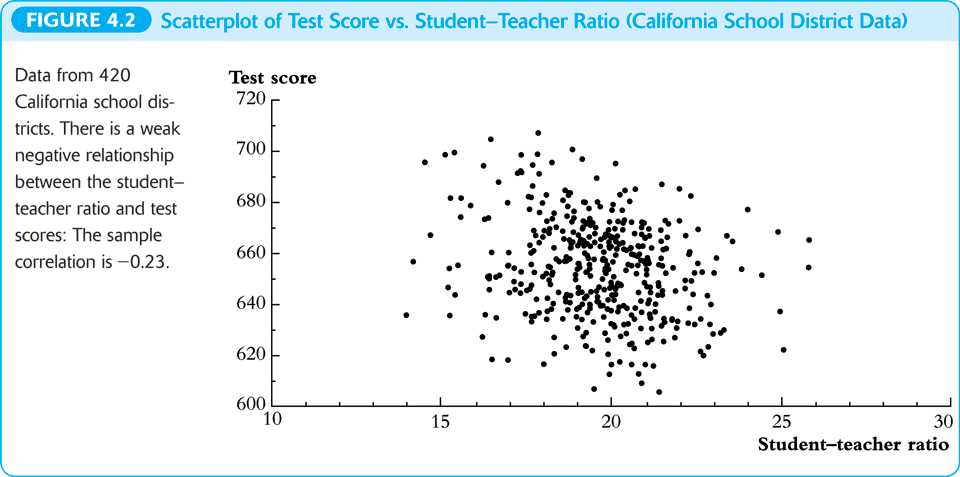
\includegraphics[width=1.0\textwidth]{figure/fig-4-2.png}
\end{center}

\begin{itemize}
\item The correlation coefficient between the two variables is -0.23.
\end{itemize}
\end{frame}

\begin{frame}[label={sec:org321a586}]{Regression analysis}
$$\widehat{TestScore} = 698.93 - 2.28 \times STR$$

\begin{figure}[htbp]
\centering
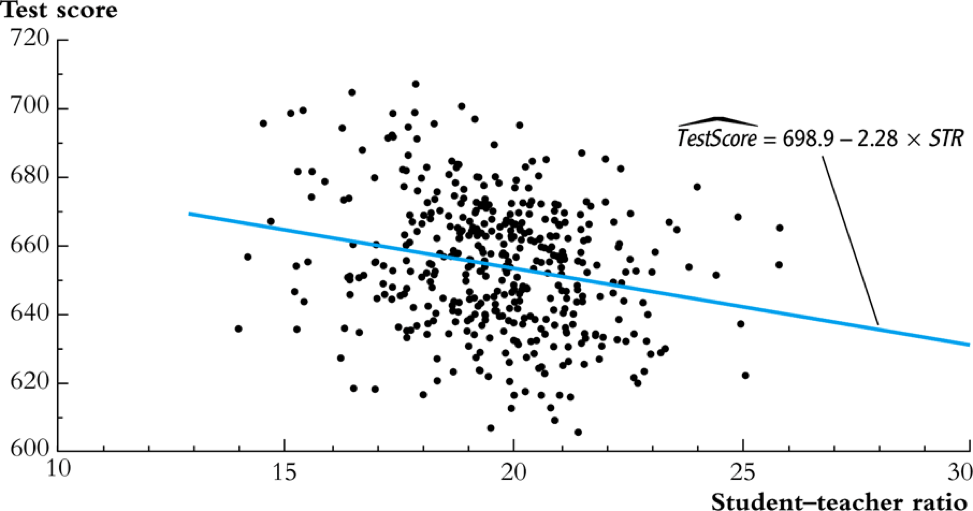
\includegraphics[width=0.85\textwidth]{figure/fig-4-3.png}
\end{figure}
\end{frame}

\begin{frame}[label={sec:org52a7dd3}]{Interpretation of the estimated coefficients}
\begin{itemize}
\item What does the slope tell us?

\item How large is the effect actually?

\item What does the intercept mean?
\end{itemize}
\end{frame}


\section{The Algebraic Properties of the OLS Estimator}
\label{sec:orgaeafd08}

\begin{frame}[label={sec:orgbe61641}]{The algebraic properties of the ols estimator}
\begin{itemize}
\item Let's first look at some of the algebraic properties of the OLS
estimators.
\item These properties hold regardless of any statistical assumptions.
\end{itemize}
\end{frame}

\begin{frame}[label={sec:org34481d2}]{TSS, ESS, and SSR}
\begin{itemize}
\item From \(Y_i = \hat{Y}_i + \hat{u}_i\), we can define
\item \alert{The total sum of squares}: \(TSS = \sum_{i=1}^n (Y_i - \overline{Y})^2\)
\item \alert{The explained sum of squares}: \(ESS = \sum_{i=1}^n (\hat{Y}_i - \overline{Y})^2\)
\item \alert{The sum of squared residuals}: \(SSR = \sum_{i=1}^n (Y_i -
  \hat{Y}_i)^2 = \sum_{i=1}^n \hat{u}_i^2\)
\item The "deviation from the mean" form is only valid when an intercept
is included in the regression model.
\end{itemize}
\end{frame}

\begin{frame}[label={sec:org1aedfbf}]{Some algebraic properties among \(\hat{u}_i\), \(\hat{Y}_i\), and \(Y_i\)}
\begin{gather}
\sum_{i=1}^n \hat{u}_i = 0 \label{eq:algebra-ols-1} \\
\frac{1}{n} \sum_{i=1}^n \hat{Y}_i = \overline{Y} \label{eq:algebra-ols-2} \\
\sum_{i=1}^n \hat{u}_i X_i = 0 \label{eq:algebra-ols-3} \\
TSS = ESS + SSR \label{eq:tss-ess}
\end{gather}
\end{frame}

\begin{frame}[label={sec:org21ef9d3}]{Proof of \(\sum_{i=1}^n \hat{u}_i = 0\)}
\[\hat{u}_i = Y_i - \hat{\beta}_0 - \hat{\beta}_1 X_i = (Y_i -
\overline{Y}) - \hat{\beta}_1 (X_i - \overline{X})\]

\[\sum_{i=1}^n \hat{u}_i = \sum_{i=1}^n (Y_i - \overline{Y}) -
\hat{\beta}_1 \sum_{i=1}^n (X_i - \overline{X}) = 0\]
\end{frame}

\begin{frame}[label={sec:org4e9928f}]{Proof of \(\frac{1}{n} \sum_{i=1}^n \hat{Y}_i = \overline{Y}\)}
Note that \(Y_i = \hat{Y}_i + \hat{u}_i\). So
\[\sum_{i=1}^n Y_i =
\sum_{i=1}^n \hat{Y}_i + \sum_{i=1}^n \hat{u}_i = \sum_{i=1}^n
\hat{Y}_i\]
It follows that \(\overline{\hat{Y}} = (1/n)\sum_{i=1}^n \hat{Y}_i = \overline{Y}\).
\end{frame}

\begin{frame}[label={sec:org28d3841}]{Proof of \(\sum_{i=1}^n \hat{u}_i X_i = 0\)}
\begin{align*}
& \sum_{i=1}^n \hat{u}_i X_i \\
=& \sum_{i=1}^n \hat{u}_i (X_i - \overline{X}) \\
=& \sum_{i=1}^n \left[ (Y_i - \overline{Y}) - \hat{\beta}_1 (X_i - \overline{X}) \right] (X_i - \overline{X}) \\
=& \sum_{i=1}^n (X_i - \overline{X})(Y_i - \overline{Y}) - \hat{\beta}_1 \sum_{i=1}^n (X_i -\overline{X})^2 = 0
\end{align*}
\end{frame}

\begin{frame}[label={sec:org07aa692}]{Proof of \(TSS = ESS + SSR\)}
\begin{equation*}
\begin{split}
TSS &= \sum_{i=1}^n (Y_i - \overline{Y})^2 = \sum_{i=1}^n (Y_i - \hat{Y}_i + \hat{Y}_i - \overline{Y})^2 \\
&= \sum_{i=1}^n (Y_i - \hat{Y}_i)^2 + \sum_{i=1}^n (\hat{Y}_i - \overline{Y})^2 + 2\sum_{i=1}^n (Y_i - \hat{Y}_i)(\hat{Y}_i - \overline{Y}) \\
&= SSR + ESS + 2\sum_{i=1}^n \hat{u}_i \hat{Y}_i \\
&= SSR + ESS + 2\sum_{i=1}^n \hat{u}_i(\hat{\beta}_0 + \hat{\beta}_1 X_i) \\
&= SSR + ESS
\end{split}
\end{equation*}
\end{frame}








\section{Measures of Fit}
\label{sec:org2f06e59}

\begin{frame}[label={sec:org2fd339b}]{Goodness of Fit: R\(^{\text{2}}\)}
\begin{equation}
\label{eq:rsquared}
R^2 = \frac{ESS}{TSS} = 1 - \frac{SSR}{TSS}
\end{equation}

\begin{itemize}
\item \(R^2\) is often called the coefficient of determination.
\item It indicates the proportion of the variance in the dependent
variable that is predictable from the independent variable(s).
\end{itemize}
\end{frame}

\begin{frame}[label={sec:orgdb12c94}]{\(R^2 \in [0, 1]\)}
\begin{itemize}
\item \(R^2 = 0\) when \(\hat{\beta}_1 = 0\).
\begin{align*}
\hat{\beta}_1 = 0 &\Rightarrow Y_i = \hat{\beta}_0 + \hat{u}_i
\Rightarrow \hat{Y}_i = \overline{Y} = \hat{\beta}_0 \\ 
&\Rightarrow ESS
= \sum_i^n (\hat{Y}_i - \overline{Y})^2 = 0 \Rightarrow R^2 = 0
\end{align*}
\item \(R^2 = 1\) when \(\hat{u}_i = 0\) for all \(i = 1, \ldots, n\).
\[ \hat{u}_i = 0 \Rightarrow SSR = \sum_i^n \hat{u}_i^2 = 0
  \Rightarrow R^2 = 1 \]
\end{itemize}
\end{frame}

\begin{frame}[label={sec:orgce96dc9}]{\(R^2 = r^2_{XY}\)}
\begin{itemize}
\item \(r_{XY}\) is the sample correlation coefficient
\[ r_{XY} = \frac{S_{XY}}{S_X S_Y} = \frac{\sum_i^n(X_i -
  \overline{X})(Y_i - \overline{Y})}{\left[\sum_i^n (X_i - \overline{X})^2 \sum_i^n (Y_i -
  \overline{Y})^2 \right]^{1/2}} \]
\end{itemize}
\end{frame}

\begin{frame}[label={sec:org03a1aa8}]{\(R^2 = r^2_{XY}\) (cont'd)}
\begin{align*}
ESS &= \sum_{i=1}^n (\hat{Y}_i - \overline{Y})^2 = \sum_{i=1}^n (\hat{\beta}_0 + \hat{\beta}_1 X_i - \overline{Y})^2 \\
&= \sum_{i=1}^n (\overline{Y} - \hat{\beta}_1 \overline{X} + \hat{\beta}_1 X_i - \overline{Y})^2 \\
&= \sum_{i=1}^n \left[ \hat{\beta}_1 (X_i - \overline{X}) \right]^2 = \hat{\beta}_1^2 \sum_{i=1}^n (X_i - \overline{X})^2 \\
&= \left[\frac{\sum_{i=1}^n (X_i - \overline{X})(Y_i - \overline{Y})}{\sum_{i=1}^n (X_i - \overline{X})^2}\right]^2 \sum_{i=1}^n (X_i - \overline{X})^2 \\
&= \frac{\left[ \sum_{i=1}^n (X_i - \overline{X})(Y_i - \overline{Y}) \right]^2}{\sum_{i=1}^n (X_i - \overline{X})^2}
\end{align*}
\end{frame}

\begin{frame}[label={sec:orgf10fd61}]{\(R^2 = r^2_{XY}\) (cont'd)}
\begin{itemize}
\item It follows that
\[
  R^2 = \frac{SSR}{TSS} = \frac{\left[ \sum_{i=1}^n (X_i - \overline{X})(Y_i - \overline{Y}) \right]^2}{\sum_{i=1}^n (X_i - \overline{X})^2 \sum_{i=1}^n (Y_i - \overline{Y})^2} = r^2_{XY}
  \]

\item \emph{Note}: This property holds only for the linear regression model
with \alert{one regressor and an intercept}.
\end{itemize}
\end{frame}

\begin{frame}[label={sec:orga8f8e18}]{The use of \(R^2\)}
\begin{itemize}
\item \(R^2\) is usually the first statistics that we look at for judging
how well the regression model fits the data.

\item However, we cannot merely rely on \(R^2\) for judge whether the
regression model is "good" or "bad".
\end{itemize}
\end{frame}

\begin{frame}[label={sec:orgd1a92a7}]{The standard error of regression (SER) as a measure of fit}
\begin{equation}
\label{eq:ser}
\mathrm{SER} = \sqrt{\frac{1}{n-2}\sum^n_{i=1} \hat{u}_i^2} = s
\end{equation}

\begin{itemize}
\item SER has the same unit of \(u_i\), which are the unit of \(Y_i\).
\item SER measures the average “size” of the OLS residual.
\item The root mean squared error (RMSE) is closely related to the SER:
\[ \mathrm{RMSE} = \sqrt{\frac{1}{n}\sum^n_{i=2} \hat{u}_i^2} \]
As \(n \rightarrow \infty\), \(SER = RMSE\).
\end{itemize}
\end{frame}

\begin{frame}[label={sec:orgc9129e1}]{\(R^2\) and SER for the application of test scores v.s. class sizes}
\begin{itemize}
\item In the application of test scores v.s. class sizes, \(R^2\) is 0.051
or 5.1\%, which implies that the regressor \emph{STR} explains only 5.1\%
of the variance of the dependent variable \emph{TestScore}.

\item SER is 18.6, which means that standard deviation of the regression
residuals is 18.6 points on the test.
\end{itemize}
\end{frame}



\section{The Least Squares Assumptions}
\label{sec:orgd5e4111}

\begin{frame}[label={sec:org182b352}]{Assumption 1: The conditional mean of \(u_i\) given \(X_i\) is zero}
\begin{equation}
\label{eq:Eu}
E(u_i | X_i) = 0
\end{equation}

\begin{itemize}
\item If the equation above is satisfied, then \(X_i\) is called
\alert{exogenous}.
\item This assumption can be stated a little stronger as \(E(u|X=x) = 0\)
for any value \(x\), that is \(E(u_i | X_1, \ldots, X_n) = 0\).
\item It follows that \(E(u)=E(E(u|X))=E(0)=0\).
\end{itemize}
\end{frame}

\begin{frame}[label={sec:orgffc035b}]{An illustration of Assumption 1}
\begin{figure}[htbp]
\centering
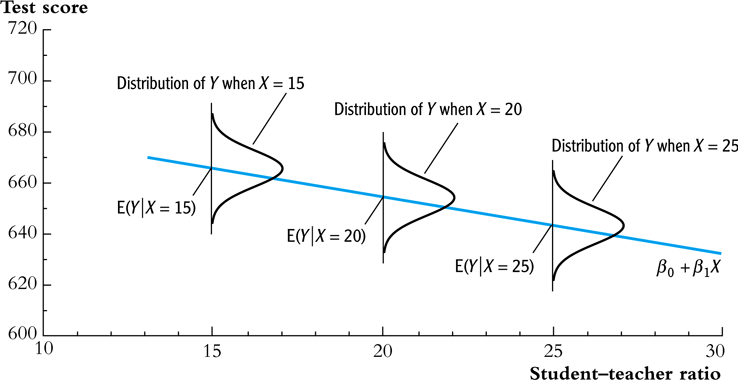
\includegraphics[width=0.7\textwidth]{figure/fig-4-4.png}
\caption{\label{fig:orga68ad0c}
An illustration of \(E(u|X=x)=0\)}
\end{figure}
\end{frame}

\begin{frame}[label={sec:org44ca875}]{Correlation and conditional mean}
\[ E(u_i | X_i) = 0 \Rightarrow \mathrm{Cov}(u_i, X_i) = 0 \]

\begin{itemize}
\item A simple proof:
\begin{equation*}
\begin{split}
\mathrm{Cov}(u_i, X_i) &= E(u_i X_i) - E(u_i) E(X_i) \\
&= E(X_i E(u_i|X_i)) - 0 \cdot E(X_i) \\
&= 0
\end{split}
\end{equation*}
where the law of iterated expectation is used twice at the second equality.

It follows that $$\mathrm{Cov}(u_i, X_i) \neq 0 \Rightarrow E(u_i|X_i) \neq 0$$
\end{itemize}
\end{frame}

\begin{frame}[label={sec:orgb2805b5}]{Assumption 2: \((X_i, Y_i)\) for \(i = 1, \ldots, n\) are i.i.d.}
\begin{itemize}
\item Each pair of \(X\) and \(Y\), i.e., \((X_i, Y_i)\) for \(i=1, \ldots, n\), is
selected randomly from the same joint distribution of \(X\) and \(Y\).
\item Since \(u_i = Y_i - \beta_0 - \beta_1 X_i\), \(u_{i}\) is i.i.d., too.
\item The cases that may violate of the i.i.d. assumption:
\begin{itemize}
\item Time series data, \(\mathrm{Cov}(Y_t, Y_{t-1}) \neq 0\). Serial
correlation problem.
\item Spatial data, \(\mathrm{Cov}(Y_r, Y_s) \neq 0\), where \(s\) and \(r\)
refer to two neighboring regions. Spatial correlation problem.
\end{itemize}
\end{itemize}
\end{frame}

\begin{frame}[label={sec:orga31eb50}]{Assumption 3: large outliers are unlikely}
$$0 < E(X^4_i) < \infty \text{ and } 0 < E(Y_i^4) < \infty$$

\begin{itemize}
\item A large outlier is an extreme value of \(X\) or \(Y\).
\item On a technical level, if \(X\) and \(Y\) are bounded, then they have finite
fourth moments, i.e., finite kurtosis.
\item The essence of this assumption is to say that a large outlier can
strongly influence the results. So we need to rule out large
outliers in estimation.
\end{itemize}
\end{frame}

\begin{frame}[label={sec:org30db89c}]{The influential observations and the leverage effects}
\begin{figure}[htbp]
\centering
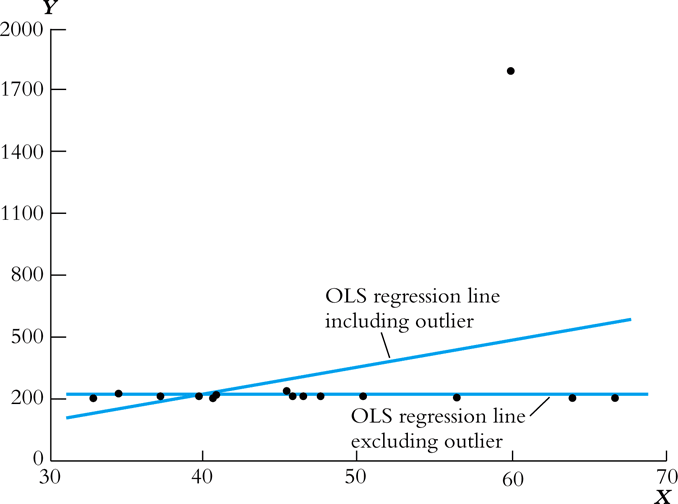
\includegraphics[width=0.7\textwidth]{figure/fig-4-5.png}
\caption{\label{fig:org2249728}
How an outlier can influence the OLS estimates}
\end{figure}
\end{frame}


\section{Sampling Distribution of the OLS Estimators}
\label{sec:orgab79fe2}

\begin{frame}[label={sec:orgb26fc70}]{Unbiasedness}
\begin{block}{The randomness of \(\hat{\beta}_0\) and \(\hat{\beta}_1\)}
Since \((X_i, Y_i)\) for \(i = 1, \ldots, n\) are randomly drawn from a
population, different draws can render different estimates, giving
rise to the randomness of \(\hat{\beta}_0\) and \(\hat{\beta}_1\).
\end{block}

\begin{block}{The unbiasedness of \(\hat{\beta}_0\) and \(\hat{\beta}_1\)}
\begin{itemize}
\item Let the true values of the intercept and the slope be \(\beta_0\) and \(\beta_1\). Based on the least squares assumption \#1: \(E(u_i|X_i) = 0\)
\[ E(\hat{\beta}_0) = \beta_0 \text{ and } E(\hat{\beta}_1) =
  \beta_1 \]
\end{itemize}
\end{block}
\end{frame}

\begin{frame}[label={sec:org7e358a0}]{Show that \(\hat{\beta}_1\) is unbiased}
\[\hat{\beta}_1  = \frac{\sum_{i=1}^n (X_i - \overline{X})(Y_i - \overline{Y})}{\sum_{i=1}^n (X_i - \overline{X})^2}\]

\begin{itemize}
\item Given the random samples \((X_i, Y_i)\) for \(i=1, \ldots, n\), from
$$Y_i = \beta_0 + \beta_1 X_i + u_i$$
We know that 
$$\overline{Y} = \beta_0 + \beta_1 \overline{X} + \bar{u}$$
It follows that 
$$Y_i - \overline{Y} = \beta_1 (X_i - \overline{X}) + u_i - \overline{u}$$
\end{itemize}
\end{frame}

\begin{frame}[shrink,label={sec:orgec871ca}]{Show that \(\hat{\beta}_1\) is unbiased (cont'd)}
\begin{itemize}
\item The numerator in \(\hat{\beta}_1\) is
\begin{equation*}
\begin{split}
& \sum_i (X_i - \overline{X})(Y_i - \overline{Y}) \\
&= \sum_i (X_i - \overline{X})\left[\beta_1(X_i - \overline{X}) + (u_i - \overline{u}) \right] \\
&= \beta_1 \sum_i(X_i - \overline{X})^2 + \sum_i (X_i - \overline{X})u_i - \overline{u}\sum_i (X_i - \overline{X}) \\
&= \beta_1 \sum_i(X_i - \overline{X})^2 + \sum_i (X_i - \overline{X})u_i
\end{split}
\end{equation*}

\item In the second equality, we use the fact that \(\sum_i (X_i -
  \overline{X}) = 0\).

\item Note that although we know from the first OLS
assumption, \(E(u_i) = 0\), we cannot guarantee that \(\bar{u} = 0\)
since \(u_1, \ldots, u_n\) are simply random draws of \(u_i\).
\end{itemize}
\end{frame}

\begin{frame}[label={sec:orgc3b8360}]{Show that \(\hat{\beta}_1\) is unbiased (cont'd)}
\begin{equation}
\label{eq:betahat-1b}
\hat{\beta}_1 = \beta_1 + \frac{\frac{1}{n}\sum_i (X_i - \overline{X})u_i}{\frac{1}{n}\sum_i (X_i - \overline{X})^2}
\end{equation}

\begin{itemize}
\item Then
\begin{equation*}
\begin{split}
E(\hat{\beta}_1 | X_1, \ldots, X_n) &= \beta_1 + E\left\lbrace \left[\frac{\frac{1}{n}\sum_i (X_i - \overline{X})u_i}{\frac{1}{n}\sum_i (X_i - \overline{X})^2} \right] \mid X_1, \ldots, X_n \right\rbrace \\
&= \beta_1 + \frac{\frac{1}{n}\sum_i (X_i - \overline{X})E(u_i|X_1, \ldots, X_n)}{\frac{1}{n}\sum_i (X_i - \overline{X})^2} \\
&= \beta_1\: \text{ (by assumption 1)}
\end{split}
\end{equation*}
\end{itemize}
\end{frame}

\begin{frame}[label={sec:org72a424c}]{Show that \(\hat{\beta}_1\) is unbiased (cont'd)}
\begin{itemize}
\item It follows that \[E(\hat{\beta}_1) = E(E(\hat{\beta}_1 | X_1, \ldots, X_n)) = \beta_1\]

\item Therefore, \(\hat{\beta}_1\) is an unbiased estimator of \(\beta_1\).

\item The proof of unbiasedness of \(\hat{\beta}_0\) is left for exercise.
\end{itemize}
\end{frame}

\begin{frame}[label={sec:org9b36b7b}]{The consistency of \(\hat{\beta}_0\) and \(\hat{\beta}_1\)}
\begin{itemize}
\item \(\hat{\beta}\) is said to be a consistent estimator
of \(\beta\) if as \(n\) goes to infinity, \(\hat{\beta}\) is in probability
close to \(\beta\), which can be denoted as \(n \rightarrow \infty,
  \hat{\beta} \xrightarrow{ \text{ p } } \beta\).

\item Recall the law of large number states that for random i.i.d. samples \(x_1,
  \ldots, x_n\), if \(E(x_i) = \mu\) and \(\mathrm{Var}(x_i) < \infty\), then
\(\bar{x} \xrightarrow{\text{ p }} \mu\) as \(n \rightarrow \infty\).

\item Then we can show that \(n \rightarrow \infty\),  \(\hat{\beta}
  \xrightarrow{ \text{ p } } \beta\), i.e., \(\hat{\beta}_1\) is a
consistent estimator of \(\beta_1\).
\end{itemize}
\end{frame}

\begin{frame}[label={sec:orgd8335d5}]{The asymptotic normal distribution of \(\hat{\beta}_1\)}
\begin{itemize}
\item Recall the central limit theory states that if \(X_1, \ldots, X_n\) with the mean
\(\mu\) and the variance \(0 < \sigma^2 < \infty\). Then,
$$\frac{1}{n}\sum_i X_i \xrightarrow{\text{d}}
  N(\mu, \frac{\sigma^2}{n})$$

\item We can prove that \(\hat{\beta}_1\) is asymptotically normally
distributed as 
\[ \hat{\beta}_1 \xrightarrow{ \text{d}} N\left( \beta_1,
  \sigma^2_{\hat{\beta}_1}\right) \] 
where
\begin{equation*}
\sigma^2_{\hat{\beta}_1} = \frac{1}{n}\frac{\mathrm{Var}\left((X_i - \overline{X})u_i\right)}{\mathrm{Var}(X_i)^2}
\end{equation*}

\item As \(\mathrm{Var}(X_i)\) increases, \(\mathrm{Var}(\hat{\beta}_1)\) decreases.

\item As \(\mathrm{Var}(u_i)\) increases, \(\mathrm{Var}(\hat{\beta}_1)\) increases.
\end{itemize}
\end{frame}

\begin{frame}[label={sec:orgfe5295c}]{The asymptotic normal distribution of \(\hat{\beta}_0\)}
\begin{itemize}
\item Similarly, we can show that 
$$\hat{\beta}_0 \xrightarrow{\text{d}} N(\beta_0,
  \sigma^2_{\hat{\beta}_0})$$
 where
\begin{equation*}
\sigma^2_{\hat{\beta}_0} = \frac{1}{n}\frac{\mathrm{Var}(H_i u_i)}{\left( E(H^2_i) \right)^2}, \text{ and }
H_i = 1 - \left( \frac{\mu_X}{E(X_i^2)} \right)X_i
\end{equation*}
\end{itemize}
\end{frame}
\end{document}